% Standalone figures for dissertation inclusion
% Required packages: pgfplots, tikz, xcolor
% Usage: % Standalone figures for dissertation inclusion
% Required packages: pgfplots, tikz, xcolor
% Usage: % Standalone figures for dissertation inclusion
% Required packages: pgfplots, tikz, xcolor
% Usage: % Standalone figures for dissertation inclusion
% Required packages: pgfplots, tikz, xcolor
% Usage: \input{evaluation_figures.tex}

% Color definitions (include if not already defined)
\ifx\infixcolor\undefined
\definecolor{infixcolor}{RGB}{31, 119, 180}
\definecolor{prefixcolor}{RGB}{255, 127, 14}
\definecolor{basecolor}{RGB}{44, 160, 44}
\definecolor{mediumcolor}{RGB}{214, 39, 40}
\definecolor{largecolor}{RGB}{148, 103, 189}
\fi

%==============================================================================
% FIGURE 1: Model Comparison Bar Chart
%==============================================================================
\begin{figure}[htbp]
\centering
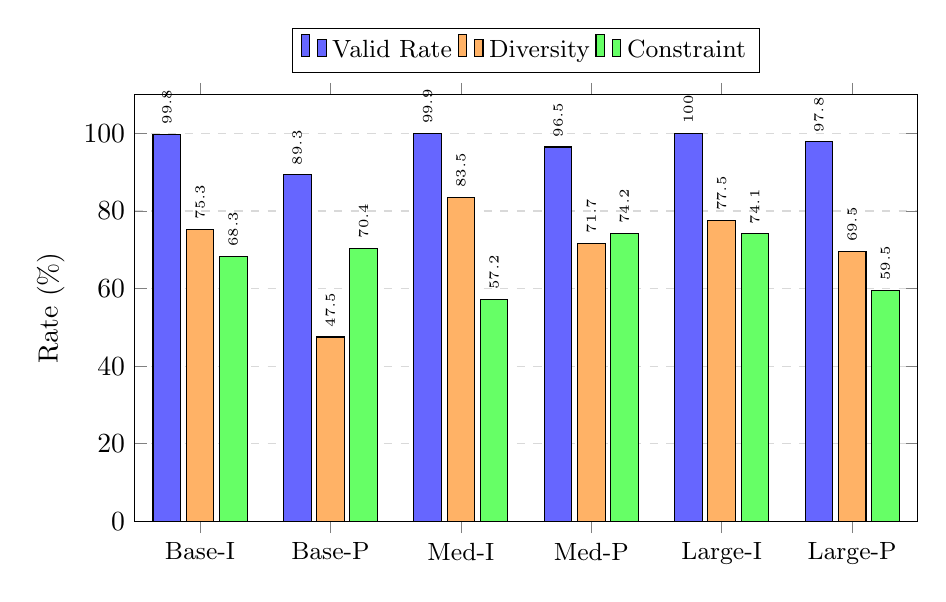
\begin{tikzpicture}
\begin{axis}[
    ybar,
    bar width=10pt,
    width=0.95\textwidth,
    height=7cm,
    ylabel={Rate (\%)},
    symbolic x coords={Base-I, Base-P, Med-I, Med-P, Large-I, Large-P},
    xtick=data,
    x tick label style={font=\small},
    ymin=0, ymax=110,
    legend style={at={(0.5,1.05)}, anchor=south, legend columns=3, font=\small},
    nodes near coords,
    nodes near coords style={font=\tiny, rotate=90, anchor=west},
    every node near coord/.append style={/pgf/number format/.cd, fixed, precision=1},
    ymajorgrids=true,
    grid style={dashed,gray!30},
]
\addplot[fill=blue!60] coordinates {
    (Base-I, 99.8) (Base-P, 89.3)
    (Med-I, 99.9) (Med-P, 96.5)
    (Large-I, 100.0) (Large-P, 97.8)
};
\addplot[fill=orange!60] coordinates {
    (Base-I, 75.3) (Base-P, 47.5)
    (Med-I, 83.5) (Med-P, 71.7)
    (Large-I, 77.5) (Large-P, 69.5)
};
\addplot[fill=green!60] coordinates {
    (Base-I, 68.3) (Base-P, 70.4)
    (Med-I, 57.2) (Med-P, 74.2)
    (Large-I, 74.1) (Large-P, 59.5)
};
\legend{Valid Rate, Diversity, Constraint}
\end{axis}
\end{tikzpicture}
\caption{Performance metrics across all model configurations. I=Infix, P=Prefix. Infix models consistently outperform prefix models in validity and diversity.}
\label{fig:model_comparison_bar}
\end{figure}

%==============================================================================
% FIGURE 2: Infix vs Prefix Comparison
%==============================================================================
\begin{figure}[htbp]
\centering
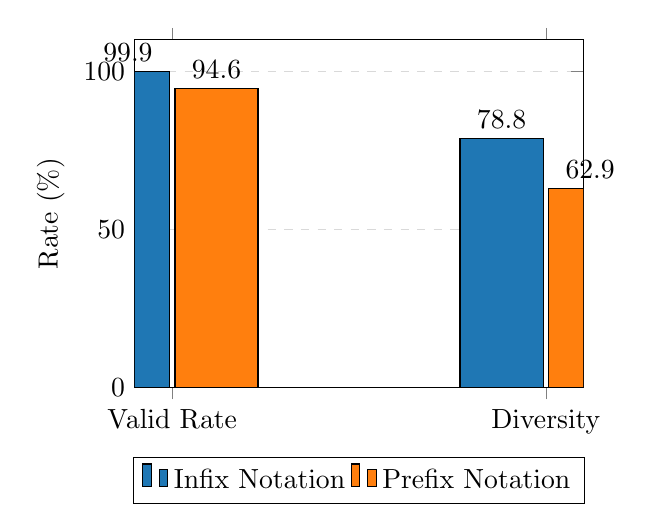
\begin{tikzpicture}
\begin{axis}[
    ybar,
    bar width=30pt,
    width=0.6\textwidth,
    height=6cm,
    ylabel={Rate (\%)},
    symbolic x coords={Valid Rate, Diversity},
    xtick=data,
    ymin=0, ymax=110,
    legend style={at={(0.5,-0.2)}, anchor=north, legend columns=2},
    nodes near coords,
    nodes near coords style={font=\normalsize, above},
    every node near coord/.append style={/pgf/number format/.cd, fixed, precision=1},
    ymajorgrids=true,
    grid style={dashed,gray!30},
]
\addplot[fill=infixcolor] coordinates {(Valid Rate, 99.9) (Diversity, 78.8)};
\addplot[fill=prefixcolor] coordinates {(Valid Rate, 94.6) (Diversity, 62.9)};
\legend{Infix Notation, Prefix Notation}
\end{axis}
\end{tikzpicture}
\caption{Notation format comparison. Infix notation achieves +5.3 pp higher valid rate and +15.9 pp higher diversity than prefix notation.}
\label{fig:notation_comparison}
\end{figure}

%==============================================================================
% FIGURE 3: Temperature Trade-off
%==============================================================================
\begin{figure}[htbp]
\centering
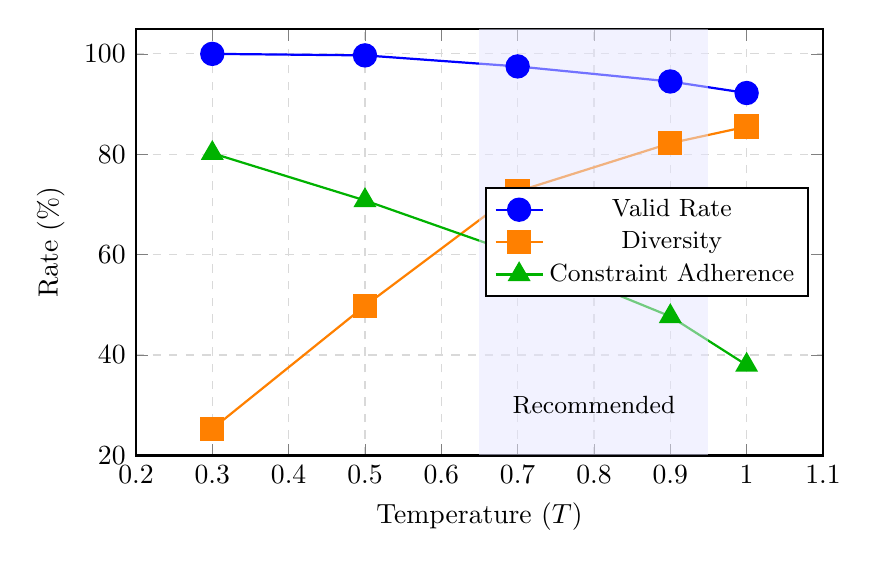
\begin{tikzpicture}
\begin{axis}[
    width=0.85\textwidth,
    height=7cm,
    xlabel={Temperature ($T$)},
    ylabel={Rate (\%)},
    xmin=0.2, xmax=1.1,
    ymin=20, ymax=105,
    legend style={at={(0.98,0.5)}, anchor=east, font=\small},
    grid=major,
    grid style={dashed,gray!30},
    mark size=4pt,
    thick,
]
\addplot[color=blue, mark=*] coordinates {
    (0.3, 100.0) (0.5, 99.7) (0.7, 97.5) (0.9, 94.5) (1.0, 92.2)
};
\addplot[color=orange, mark=square*] coordinates {
    (0.3, 25.3) (0.5, 49.8) (0.7, 72.6) (0.9, 82.2) (1.0, 85.5)
};
\addplot[color=green!70!black, mark=triangle*] coordinates {
    (0.3, 80.2) (0.5, 70.8) (0.7, 60.1) (0.9, 47.7) (1.0, 38.0)
};

% Add shaded region for recommended range
\fill[blue!10, opacity=0.5] (axis cs:0.65,20) rectangle (axis cs:0.95,105);
\node[font=\small] at (axis cs:0.8,30) {Recommended};

\legend{Valid Rate, Diversity, Constraint Adherence}
\end{axis}
\end{tikzpicture}
\caption{Temperature effect on generation quality. Shaded region ($T=0.7$--$0.9$) represents recommended operating range balancing validity and diversity.}
\label{fig:temperature_tradeoff}
\end{figure}

%==============================================================================
% FIGURE 4: Scaling Behavior
%==============================================================================
\begin{figure}[htbp]
\centering
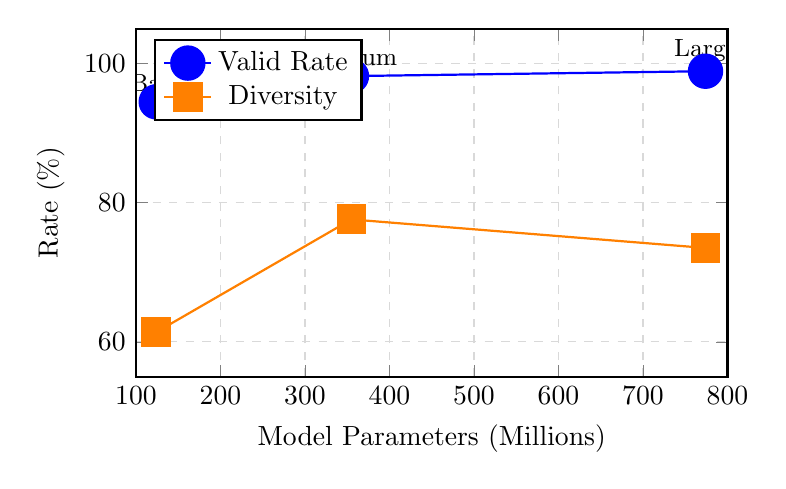
\begin{tikzpicture}
\begin{axis}[
    width=0.75\textwidth,
    height=6cm,
    xlabel={Model Parameters (Millions)},
    ylabel={Rate (\%)},
    xmin=100, xmax=800,
    ymin=55, ymax=105,
    legend style={at={(0.03,0.97)}, anchor=north west},
    grid=major,
    grid style={dashed,gray!30},
    mark size=5pt,
    thick,
]
\addplot[color=blue, mark=*, mark size=6pt] coordinates {
    (124, 94.5) (355, 98.2) (774, 98.9)
};
\addplot[color=orange, mark=square*, mark size=5pt] coordinates {
    (124, 61.4) (355, 77.6) (774, 73.5)
};
% Add labels
\node[above, font=\small] at (axis cs:124,94.5) {Base};
\node[above, font=\small] at (axis cs:355,98.2) {Medium};
\node[above, font=\small] at (axis cs:774,98.9) {Large};
\legend{Valid Rate, Diversity}
\end{axis}
\end{tikzpicture}
\caption{Model scaling behavior. Valid rate increases with model size. Diversity peaks at Medium (355M parameters).}
\label{fig:scaling}
\end{figure}

%==============================================================================
% FIGURE 5: Temperature by Model (Detailed)
%==============================================================================
\begin{figure}[htbp]
\centering
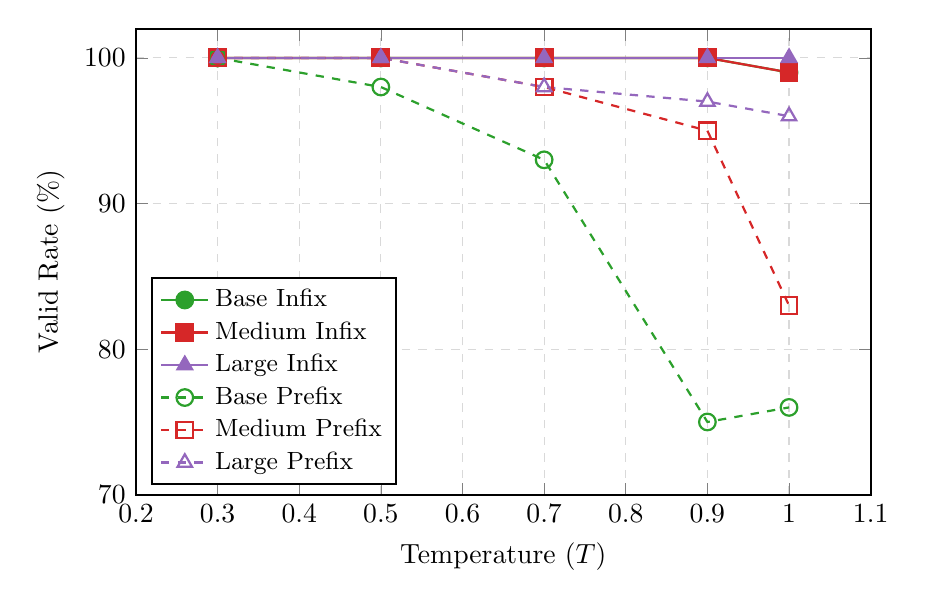
\begin{tikzpicture}
\begin{axis}[
    width=0.9\textwidth,
    height=7.5cm,
    xlabel={Temperature ($T$)},
    ylabel={Valid Rate (\%)},
    xmin=0.2, xmax=1.1,
    ymin=70, ymax=102,
    legend style={at={(0.02,0.02)}, anchor=south west, font=\small, cells={anchor=west}},
    grid=major,
    grid style={dashed,gray!30},
    mark size=3pt,
    thick,
]
% Infix models (solid lines)
\addplot[color=basecolor, mark=*] coordinates {
    (0.3, 100) (0.5, 100) (0.7, 100) (0.9, 100) (1.0, 99)
};
\addplot[color=mediumcolor, mark=square*] coordinates {
    (0.3, 100) (0.5, 100) (0.7, 100) (0.9, 100) (1.0, 99)
};
\addplot[color=largecolor, mark=triangle*] coordinates {
    (0.3, 100) (0.5, 100) (0.7, 100) (0.9, 100) (1.0, 100)
};
% Prefix models (dashed lines)
\addplot[color=basecolor, dashed, mark=o, mark options={solid}] coordinates {
    (0.3, 100) (0.5, 98) (0.7, 93) (0.9, 75) (1.0, 76)
};
\addplot[color=mediumcolor, dashed, mark=square, mark options={solid}] coordinates {
    (0.3, 100) (0.5, 100) (0.7, 98) (0.9, 95) (1.0, 83)
};
\addplot[color=largecolor, dashed, mark=triangle, mark options={solid}] coordinates {
    (0.3, 100) (0.5, 100) (0.7, 98) (0.9, 97) (1.0, 96)
};
\legend{Base Infix, Medium Infix, Large Infix, Base Prefix, Medium Prefix, Large Prefix}
\end{axis}
\end{tikzpicture}
\caption{Valid rate vs. temperature by model configuration. Solid lines represent infix models; dashed lines represent prefix models. Infix models maintain stability across temperatures.}
\label{fig:temp_by_model}
\end{figure}

%==============================================================================
% FIGURE 6: Prompt Complexity Effect
%==============================================================================
\begin{figure}[htbp]
\centering
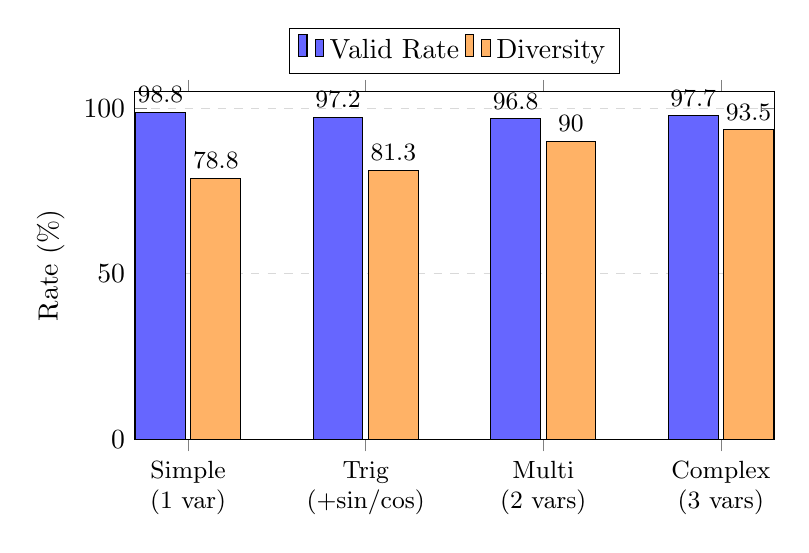
\begin{tikzpicture}
\begin{axis}[
    ybar,
    bar width=18pt,
    width=0.8\textwidth,
    height=6cm,
    ylabel={Rate (\%)},
    symbolic x coords={Simple, Trig, Multi, Complex},
    xtick=data,
    xticklabels={Simple\\(1 var), Trig\\(+sin/cos), Multi\\(2 vars), Complex\\(3 vars)},
    x tick label style={align=center, font=\small},
    ymin=0, ymax=105,
    legend style={at={(0.5,1.05)}, anchor=south, legend columns=2},
    nodes near coords,
    nodes near coords style={font=\small},
    every node near coord/.append style={/pgf/number format/.cd, fixed, precision=1},
    ymajorgrids=true,
    grid style={dashed,gray!30},
]
\addplot[fill=blue!60] coordinates {
    (Simple, 98.8) (Trig, 97.2) (Multi, 96.8) (Complex, 97.7)
};
\addplot[fill=orange!60] coordinates {
    (Simple, 78.8) (Trig, 81.3) (Multi, 90.0) (Complex, 93.5)
};
\legend{Valid Rate, Diversity}
\end{axis}
\end{tikzpicture}
\caption{Effect of prompt complexity on generation quality. More variables and operators increase expression diversity with minimal impact on validity.}
\label{fig:prompt_complexity}
\end{figure}

%==============================================================================
% FIGURE 7: Validity-Diversity Pareto Front
%==============================================================================
\begin{figure}[htbp]
\centering
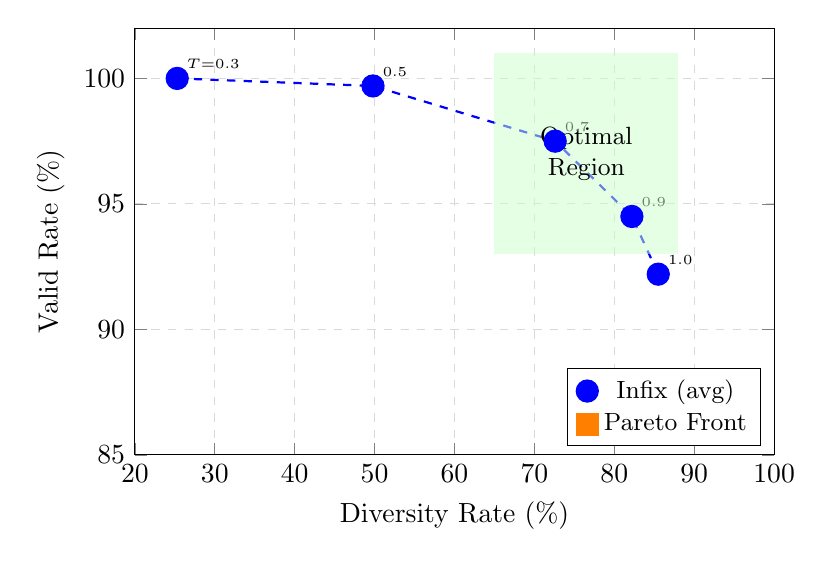
\begin{tikzpicture}
\begin{axis}[
    width=0.8\textwidth,
    height=7cm,
    xlabel={Diversity Rate (\%)},
    ylabel={Valid Rate (\%)},
    xmin=20, xmax=100,
    ymin=85, ymax=102,
    legend style={at={(0.98,0.02)}, anchor=south east, font=\small},
    grid=major,
    grid style={dashed,gray!30},
    scatter/classes={
        infix={mark=*, blue},
        prefix={mark=square*, orange}
    },
]
% Infix models at different temperatures
\addplot[scatter, only marks, scatter src=explicit symbolic, mark size=4pt]
coordinates {
    (25.3, 100.0) [infix]  % T=0.3
    (49.8, 99.7) [infix]   % T=0.5
    (72.6, 97.5) [infix]   % T=0.7
    (82.2, 94.5) [infix]   % T=0.9
    (85.5, 92.2) [infix]   % T=1.0
};
% Labels for temperatures
\node[font=\tiny, above right] at (axis cs:25.3,100) {$T$=0.3};
\node[font=\tiny, above right] at (axis cs:49.8,99.7) {0.5};
\node[font=\tiny, above right] at (axis cs:72.6,97.5) {0.7};
\node[font=\tiny, above right] at (axis cs:82.2,94.5) {0.9};
\node[font=\tiny, above right] at (axis cs:85.5,92.2) {1.0};

% Draw Pareto front
\addplot[blue, thick, dashed, no markers] coordinates {
    (25.3, 100.0) (49.8, 99.7) (72.6, 97.5) (82.2, 94.5) (85.5, 92.2)
};

% Highlight optimal region
\fill[green!20, opacity=0.5] (axis cs:65,93) rectangle (axis cs:88,101);
\node[font=\small, align=center] at (axis cs:76.5,97) {Optimal\\Region};

\legend{Infix (avg), Pareto Front}
\end{axis}
\end{tikzpicture}
\caption{Validity-diversity trade-off across temperature settings. The Pareto front shows the optimal trade-off achievable. Green region indicates recommended operating range.}
\label{fig:pareto}
\end{figure}

%==============================================================================
% FIGURE 8: Heatmap - Valid Rate by Model and Temperature
%==============================================================================
\begin{figure}[htbp]
\centering
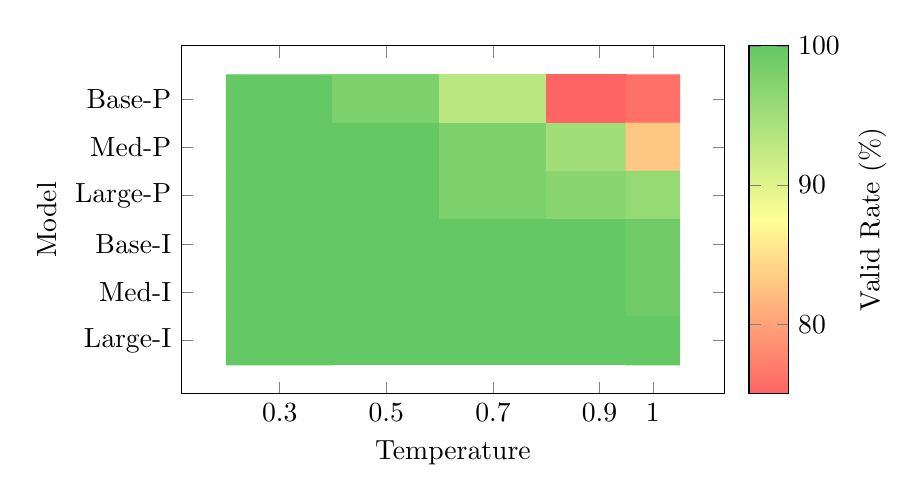
\begin{tikzpicture}
\begin{axis}[
    view={0}{90},
    colormap={validmap}{
        rgb255(0cm)=(255,100,100);
        rgb255(0.5cm)=(255,255,150);
        rgb255(1cm)=(100,200,100)
    },
    colorbar,
    colorbar style={
        ylabel={Valid Rate (\%)},
    },
    point meta min=75,
    point meta max=100,
    xlabel={Temperature},
    ylabel={Model},
    xtick={0.3, 0.5, 0.7, 0.9, 1.0},
    ytick={1,2,3,4,5,6},
    yticklabels={Base-P, Med-P, Large-P, Base-I, Med-I, Large-I},
    width=0.7\textwidth,
    height=6cm,
]
\addplot[
    matrix plot,
    mesh/cols=5,
    point meta=explicit,
] table[meta=C] {
x       y   C
0.3     1   100
0.5     1   98
0.7     1   93
0.9     1   75
1.0     1   76
0.3     2   100
0.5     2   100
0.7     2   98
0.9     2   95
1.0     2   83
0.3     3   100
0.5     3   100
0.7     3   98
0.9     3   97
1.0     3   96
0.3     4   100
0.5     4   100
0.7     4   100
0.9     4   100
1.0     4   99
0.3     5   100
0.5     5   100
0.7     5   100
0.9     5   100
1.0     5   99
0.3     6   100
0.5     6   100
0.7     6   100
0.9     6   100
1.0     6   100
};
\end{axis}
\end{tikzpicture}
\caption{Heatmap of valid rate by model and temperature. Green indicates high validity ($\geq$97\%), yellow moderate (90--97\%), red lower ($<$90\%). Infix models (top 3 rows) maintain stability.}
\label{fig:heatmap}
\end{figure}


% Color definitions (include if not already defined)
\ifx\infixcolor\undefined
\definecolor{infixcolor}{RGB}{31, 119, 180}
\definecolor{prefixcolor}{RGB}{255, 127, 14}
\definecolor{basecolor}{RGB}{44, 160, 44}
\definecolor{mediumcolor}{RGB}{214, 39, 40}
\definecolor{largecolor}{RGB}{148, 103, 189}
\fi

%==============================================================================
% FIGURE 1: Model Comparison Bar Chart
%==============================================================================
\begin{figure}[htbp]
\centering
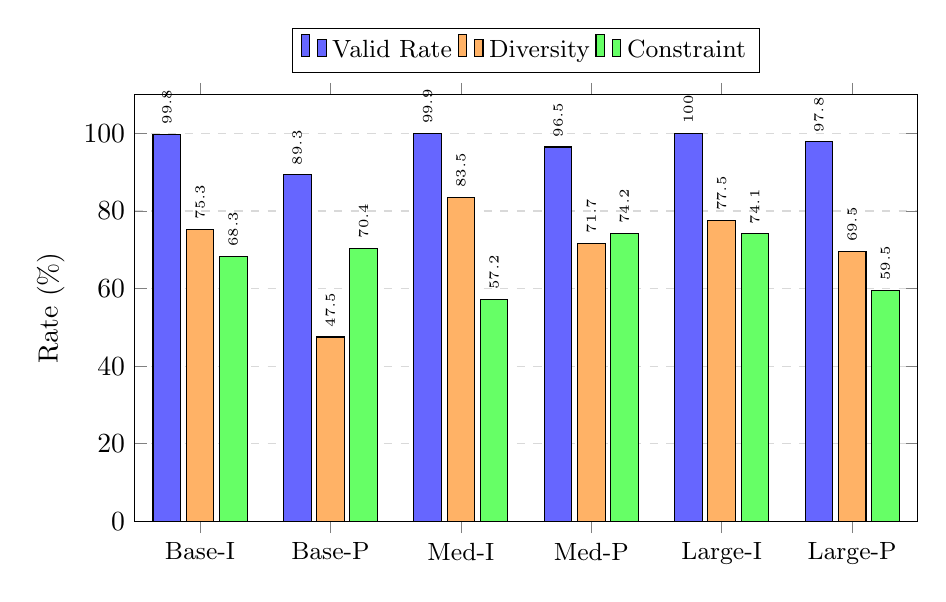
\begin{tikzpicture}
\begin{axis}[
    ybar,
    bar width=10pt,
    width=0.95\textwidth,
    height=7cm,
    ylabel={Rate (\%)},
    symbolic x coords={Base-I, Base-P, Med-I, Med-P, Large-I, Large-P},
    xtick=data,
    x tick label style={font=\small},
    ymin=0, ymax=110,
    legend style={at={(0.5,1.05)}, anchor=south, legend columns=3, font=\small},
    nodes near coords,
    nodes near coords style={font=\tiny, rotate=90, anchor=west},
    every node near coord/.append style={/pgf/number format/.cd, fixed, precision=1},
    ymajorgrids=true,
    grid style={dashed,gray!30},
]
\addplot[fill=blue!60] coordinates {
    (Base-I, 99.8) (Base-P, 89.3)
    (Med-I, 99.9) (Med-P, 96.5)
    (Large-I, 100.0) (Large-P, 97.8)
};
\addplot[fill=orange!60] coordinates {
    (Base-I, 75.3) (Base-P, 47.5)
    (Med-I, 83.5) (Med-P, 71.7)
    (Large-I, 77.5) (Large-P, 69.5)
};
\addplot[fill=green!60] coordinates {
    (Base-I, 68.3) (Base-P, 70.4)
    (Med-I, 57.2) (Med-P, 74.2)
    (Large-I, 74.1) (Large-P, 59.5)
};
\legend{Valid Rate, Diversity, Constraint}
\end{axis}
\end{tikzpicture}
\caption{Performance metrics across all model configurations. I=Infix, P=Prefix. Infix models consistently outperform prefix models in validity and diversity.}
\label{fig:model_comparison_bar}
\end{figure}

%==============================================================================
% FIGURE 2: Infix vs Prefix Comparison
%==============================================================================
\begin{figure}[htbp]
\centering
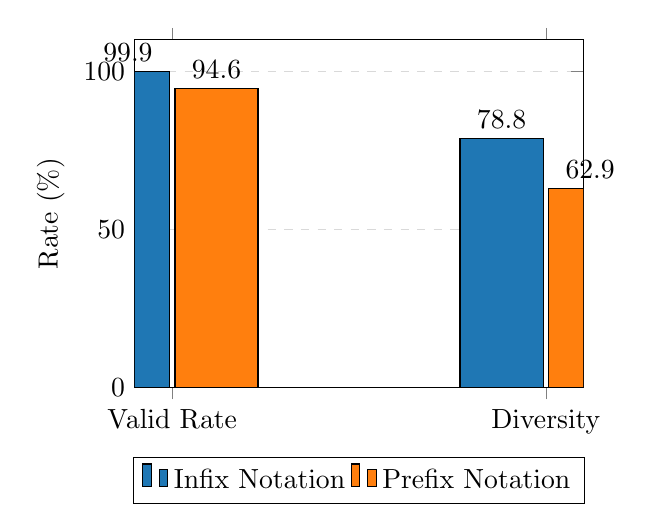
\begin{tikzpicture}
\begin{axis}[
    ybar,
    bar width=30pt,
    width=0.6\textwidth,
    height=6cm,
    ylabel={Rate (\%)},
    symbolic x coords={Valid Rate, Diversity},
    xtick=data,
    ymin=0, ymax=110,
    legend style={at={(0.5,-0.2)}, anchor=north, legend columns=2},
    nodes near coords,
    nodes near coords style={font=\normalsize, above},
    every node near coord/.append style={/pgf/number format/.cd, fixed, precision=1},
    ymajorgrids=true,
    grid style={dashed,gray!30},
]
\addplot[fill=infixcolor] coordinates {(Valid Rate, 99.9) (Diversity, 78.8)};
\addplot[fill=prefixcolor] coordinates {(Valid Rate, 94.6) (Diversity, 62.9)};
\legend{Infix Notation, Prefix Notation}
\end{axis}
\end{tikzpicture}
\caption{Notation format comparison. Infix notation achieves +5.3 pp higher valid rate and +15.9 pp higher diversity than prefix notation.}
\label{fig:notation_comparison}
\end{figure}

%==============================================================================
% FIGURE 3: Temperature Trade-off
%==============================================================================
\begin{figure}[htbp]
\centering
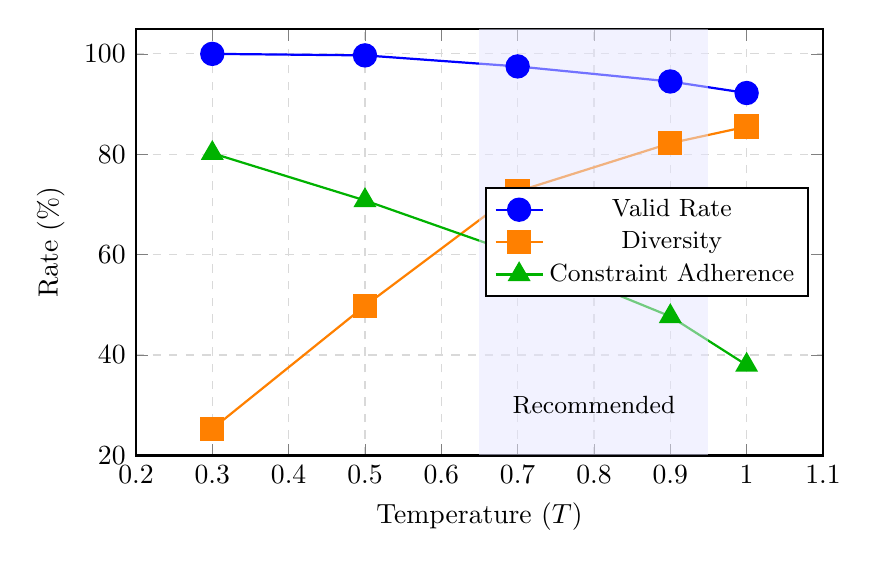
\begin{tikzpicture}
\begin{axis}[
    width=0.85\textwidth,
    height=7cm,
    xlabel={Temperature ($T$)},
    ylabel={Rate (\%)},
    xmin=0.2, xmax=1.1,
    ymin=20, ymax=105,
    legend style={at={(0.98,0.5)}, anchor=east, font=\small},
    grid=major,
    grid style={dashed,gray!30},
    mark size=4pt,
    thick,
]
\addplot[color=blue, mark=*] coordinates {
    (0.3, 100.0) (0.5, 99.7) (0.7, 97.5) (0.9, 94.5) (1.0, 92.2)
};
\addplot[color=orange, mark=square*] coordinates {
    (0.3, 25.3) (0.5, 49.8) (0.7, 72.6) (0.9, 82.2) (1.0, 85.5)
};
\addplot[color=green!70!black, mark=triangle*] coordinates {
    (0.3, 80.2) (0.5, 70.8) (0.7, 60.1) (0.9, 47.7) (1.0, 38.0)
};

% Add shaded region for recommended range
\fill[blue!10, opacity=0.5] (axis cs:0.65,20) rectangle (axis cs:0.95,105);
\node[font=\small] at (axis cs:0.8,30) {Recommended};

\legend{Valid Rate, Diversity, Constraint Adherence}
\end{axis}
\end{tikzpicture}
\caption{Temperature effect on generation quality. Shaded region ($T=0.7$--$0.9$) represents recommended operating range balancing validity and diversity.}
\label{fig:temperature_tradeoff}
\end{figure}

%==============================================================================
% FIGURE 4: Scaling Behavior
%==============================================================================
\begin{figure}[htbp]
\centering
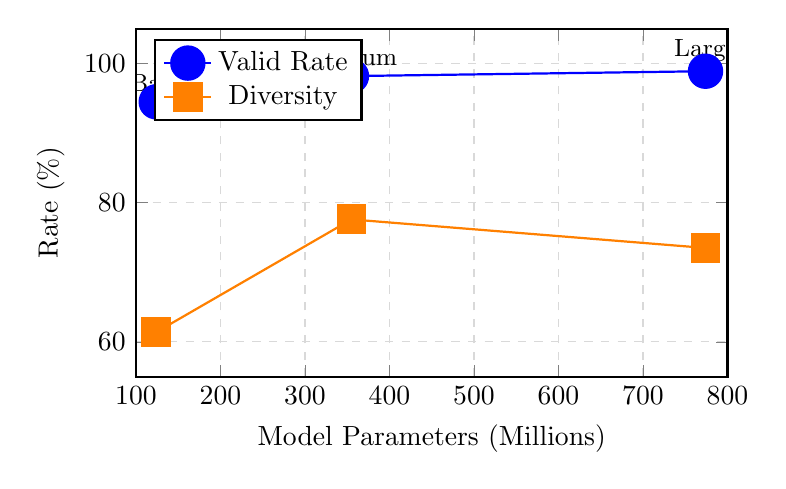
\begin{tikzpicture}
\begin{axis}[
    width=0.75\textwidth,
    height=6cm,
    xlabel={Model Parameters (Millions)},
    ylabel={Rate (\%)},
    xmin=100, xmax=800,
    ymin=55, ymax=105,
    legend style={at={(0.03,0.97)}, anchor=north west},
    grid=major,
    grid style={dashed,gray!30},
    mark size=5pt,
    thick,
]
\addplot[color=blue, mark=*, mark size=6pt] coordinates {
    (124, 94.5) (355, 98.2) (774, 98.9)
};
\addplot[color=orange, mark=square*, mark size=5pt] coordinates {
    (124, 61.4) (355, 77.6) (774, 73.5)
};
% Add labels
\node[above, font=\small] at (axis cs:124,94.5) {Base};
\node[above, font=\small] at (axis cs:355,98.2) {Medium};
\node[above, font=\small] at (axis cs:774,98.9) {Large};
\legend{Valid Rate, Diversity}
\end{axis}
\end{tikzpicture}
\caption{Model scaling behavior. Valid rate increases with model size. Diversity peaks at Medium (355M parameters).}
\label{fig:scaling}
\end{figure}

%==============================================================================
% FIGURE 5: Temperature by Model (Detailed)
%==============================================================================
\begin{figure}[htbp]
\centering
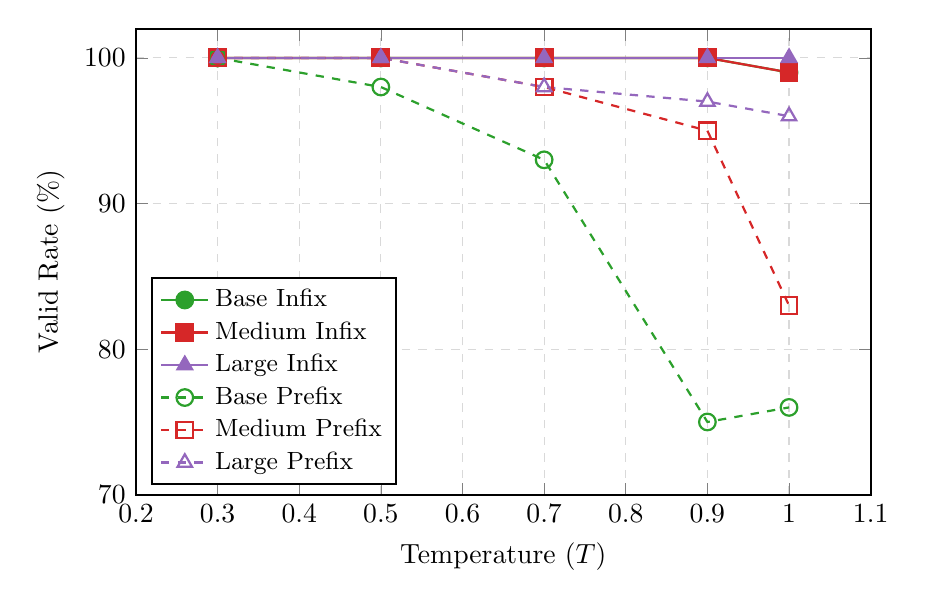
\begin{tikzpicture}
\begin{axis}[
    width=0.9\textwidth,
    height=7.5cm,
    xlabel={Temperature ($T$)},
    ylabel={Valid Rate (\%)},
    xmin=0.2, xmax=1.1,
    ymin=70, ymax=102,
    legend style={at={(0.02,0.02)}, anchor=south west, font=\small, cells={anchor=west}},
    grid=major,
    grid style={dashed,gray!30},
    mark size=3pt,
    thick,
]
% Infix models (solid lines)
\addplot[color=basecolor, mark=*] coordinates {
    (0.3, 100) (0.5, 100) (0.7, 100) (0.9, 100) (1.0, 99)
};
\addplot[color=mediumcolor, mark=square*] coordinates {
    (0.3, 100) (0.5, 100) (0.7, 100) (0.9, 100) (1.0, 99)
};
\addplot[color=largecolor, mark=triangle*] coordinates {
    (0.3, 100) (0.5, 100) (0.7, 100) (0.9, 100) (1.0, 100)
};
% Prefix models (dashed lines)
\addplot[color=basecolor, dashed, mark=o, mark options={solid}] coordinates {
    (0.3, 100) (0.5, 98) (0.7, 93) (0.9, 75) (1.0, 76)
};
\addplot[color=mediumcolor, dashed, mark=square, mark options={solid}] coordinates {
    (0.3, 100) (0.5, 100) (0.7, 98) (0.9, 95) (1.0, 83)
};
\addplot[color=largecolor, dashed, mark=triangle, mark options={solid}] coordinates {
    (0.3, 100) (0.5, 100) (0.7, 98) (0.9, 97) (1.0, 96)
};
\legend{Base Infix, Medium Infix, Large Infix, Base Prefix, Medium Prefix, Large Prefix}
\end{axis}
\end{tikzpicture}
\caption{Valid rate vs. temperature by model configuration. Solid lines represent infix models; dashed lines represent prefix models. Infix models maintain stability across temperatures.}
\label{fig:temp_by_model}
\end{figure}

%==============================================================================
% FIGURE 6: Prompt Complexity Effect
%==============================================================================
\begin{figure}[htbp]
\centering
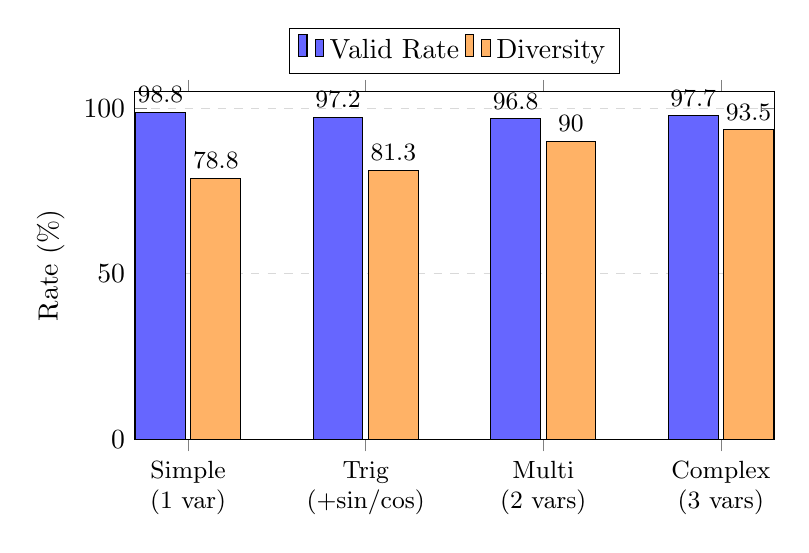
\begin{tikzpicture}
\begin{axis}[
    ybar,
    bar width=18pt,
    width=0.8\textwidth,
    height=6cm,
    ylabel={Rate (\%)},
    symbolic x coords={Simple, Trig, Multi, Complex},
    xtick=data,
    xticklabels={Simple\\(1 var), Trig\\(+sin/cos), Multi\\(2 vars), Complex\\(3 vars)},
    x tick label style={align=center, font=\small},
    ymin=0, ymax=105,
    legend style={at={(0.5,1.05)}, anchor=south, legend columns=2},
    nodes near coords,
    nodes near coords style={font=\small},
    every node near coord/.append style={/pgf/number format/.cd, fixed, precision=1},
    ymajorgrids=true,
    grid style={dashed,gray!30},
]
\addplot[fill=blue!60] coordinates {
    (Simple, 98.8) (Trig, 97.2) (Multi, 96.8) (Complex, 97.7)
};
\addplot[fill=orange!60] coordinates {
    (Simple, 78.8) (Trig, 81.3) (Multi, 90.0) (Complex, 93.5)
};
\legend{Valid Rate, Diversity}
\end{axis}
\end{tikzpicture}
\caption{Effect of prompt complexity on generation quality. More variables and operators increase expression diversity with minimal impact on validity.}
\label{fig:prompt_complexity}
\end{figure}

%==============================================================================
% FIGURE 7: Validity-Diversity Pareto Front
%==============================================================================
\begin{figure}[htbp]
\centering
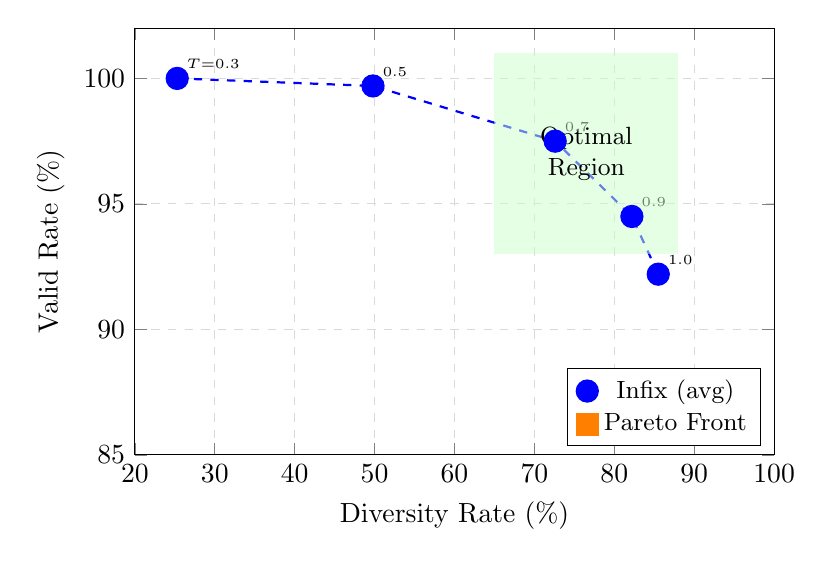
\begin{tikzpicture}
\begin{axis}[
    width=0.8\textwidth,
    height=7cm,
    xlabel={Diversity Rate (\%)},
    ylabel={Valid Rate (\%)},
    xmin=20, xmax=100,
    ymin=85, ymax=102,
    legend style={at={(0.98,0.02)}, anchor=south east, font=\small},
    grid=major,
    grid style={dashed,gray!30},
    scatter/classes={
        infix={mark=*, blue},
        prefix={mark=square*, orange}
    },
]
% Infix models at different temperatures
\addplot[scatter, only marks, scatter src=explicit symbolic, mark size=4pt]
coordinates {
    (25.3, 100.0) [infix]  % T=0.3
    (49.8, 99.7) [infix]   % T=0.5
    (72.6, 97.5) [infix]   % T=0.7
    (82.2, 94.5) [infix]   % T=0.9
    (85.5, 92.2) [infix]   % T=1.0
};
% Labels for temperatures
\node[font=\tiny, above right] at (axis cs:25.3,100) {$T$=0.3};
\node[font=\tiny, above right] at (axis cs:49.8,99.7) {0.5};
\node[font=\tiny, above right] at (axis cs:72.6,97.5) {0.7};
\node[font=\tiny, above right] at (axis cs:82.2,94.5) {0.9};
\node[font=\tiny, above right] at (axis cs:85.5,92.2) {1.0};

% Draw Pareto front
\addplot[blue, thick, dashed, no markers] coordinates {
    (25.3, 100.0) (49.8, 99.7) (72.6, 97.5) (82.2, 94.5) (85.5, 92.2)
};

% Highlight optimal region
\fill[green!20, opacity=0.5] (axis cs:65,93) rectangle (axis cs:88,101);
\node[font=\small, align=center] at (axis cs:76.5,97) {Optimal\\Region};

\legend{Infix (avg), Pareto Front}
\end{axis}
\end{tikzpicture}
\caption{Validity-diversity trade-off across temperature settings. The Pareto front shows the optimal trade-off achievable. Green region indicates recommended operating range.}
\label{fig:pareto}
\end{figure}

%==============================================================================
% FIGURE 8: Heatmap - Valid Rate by Model and Temperature
%==============================================================================
\begin{figure}[htbp]
\centering
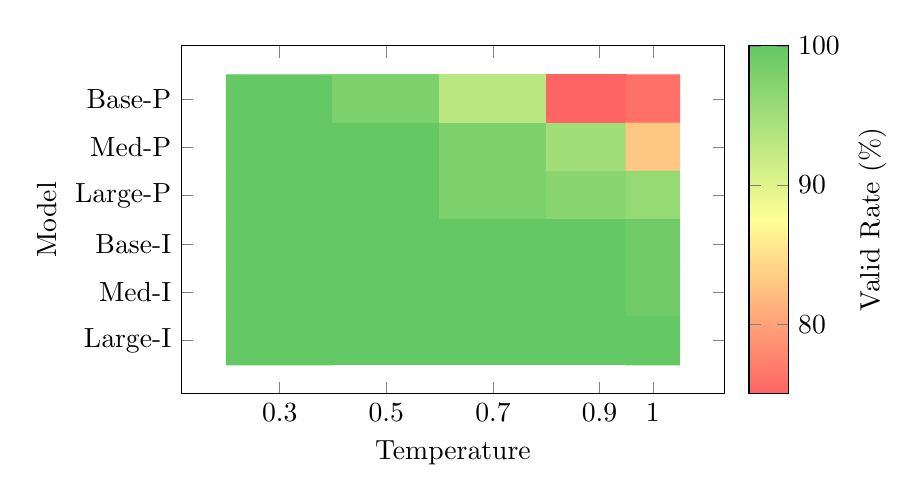
\begin{tikzpicture}
\begin{axis}[
    view={0}{90},
    colormap={validmap}{
        rgb255(0cm)=(255,100,100);
        rgb255(0.5cm)=(255,255,150);
        rgb255(1cm)=(100,200,100)
    },
    colorbar,
    colorbar style={
        ylabel={Valid Rate (\%)},
    },
    point meta min=75,
    point meta max=100,
    xlabel={Temperature},
    ylabel={Model},
    xtick={0.3, 0.5, 0.7, 0.9, 1.0},
    ytick={1,2,3,4,5,6},
    yticklabels={Base-P, Med-P, Large-P, Base-I, Med-I, Large-I},
    width=0.7\textwidth,
    height=6cm,
]
\addplot[
    matrix plot,
    mesh/cols=5,
    point meta=explicit,
] table[meta=C] {
x       y   C
0.3     1   100
0.5     1   98
0.7     1   93
0.9     1   75
1.0     1   76
0.3     2   100
0.5     2   100
0.7     2   98
0.9     2   95
1.0     2   83
0.3     3   100
0.5     3   100
0.7     3   98
0.9     3   97
1.0     3   96
0.3     4   100
0.5     4   100
0.7     4   100
0.9     4   100
1.0     4   99
0.3     5   100
0.5     5   100
0.7     5   100
0.9     5   100
1.0     5   99
0.3     6   100
0.5     6   100
0.7     6   100
0.9     6   100
1.0     6   100
};
\end{axis}
\end{tikzpicture}
\caption{Heatmap of valid rate by model and temperature. Green indicates high validity ($\geq$97\%), yellow moderate (90--97\%), red lower ($<$90\%). Infix models (top 3 rows) maintain stability.}
\label{fig:heatmap}
\end{figure}


% Color definitions (include if not already defined)
\ifx\infixcolor\undefined
\definecolor{infixcolor}{RGB}{31, 119, 180}
\definecolor{prefixcolor}{RGB}{255, 127, 14}
\definecolor{basecolor}{RGB}{44, 160, 44}
\definecolor{mediumcolor}{RGB}{214, 39, 40}
\definecolor{largecolor}{RGB}{148, 103, 189}
\fi

%==============================================================================
% FIGURE 1: Model Comparison Bar Chart
%==============================================================================
\begin{figure}[htbp]
\centering
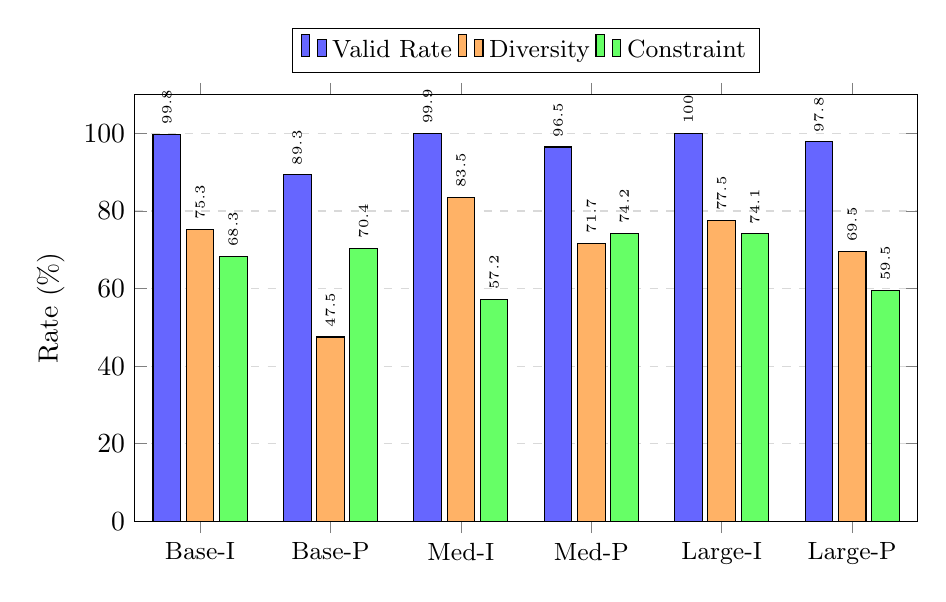
\begin{tikzpicture}
\begin{axis}[
    ybar,
    bar width=10pt,
    width=0.95\textwidth,
    height=7cm,
    ylabel={Rate (\%)},
    symbolic x coords={Base-I, Base-P, Med-I, Med-P, Large-I, Large-P},
    xtick=data,
    x tick label style={font=\small},
    ymin=0, ymax=110,
    legend style={at={(0.5,1.05)}, anchor=south, legend columns=3, font=\small},
    nodes near coords,
    nodes near coords style={font=\tiny, rotate=90, anchor=west},
    every node near coord/.append style={/pgf/number format/.cd, fixed, precision=1},
    ymajorgrids=true,
    grid style={dashed,gray!30},
]
\addplot[fill=blue!60] coordinates {
    (Base-I, 99.8) (Base-P, 89.3)
    (Med-I, 99.9) (Med-P, 96.5)
    (Large-I, 100.0) (Large-P, 97.8)
};
\addplot[fill=orange!60] coordinates {
    (Base-I, 75.3) (Base-P, 47.5)
    (Med-I, 83.5) (Med-P, 71.7)
    (Large-I, 77.5) (Large-P, 69.5)
};
\addplot[fill=green!60] coordinates {
    (Base-I, 68.3) (Base-P, 70.4)
    (Med-I, 57.2) (Med-P, 74.2)
    (Large-I, 74.1) (Large-P, 59.5)
};
\legend{Valid Rate, Diversity, Constraint}
\end{axis}
\end{tikzpicture}
\caption{Performance metrics across all model configurations. I=Infix, P=Prefix. Infix models consistently outperform prefix models in validity and diversity.}
\label{fig:model_comparison_bar}
\end{figure}

%==============================================================================
% FIGURE 2: Infix vs Prefix Comparison
%==============================================================================
\begin{figure}[htbp]
\centering
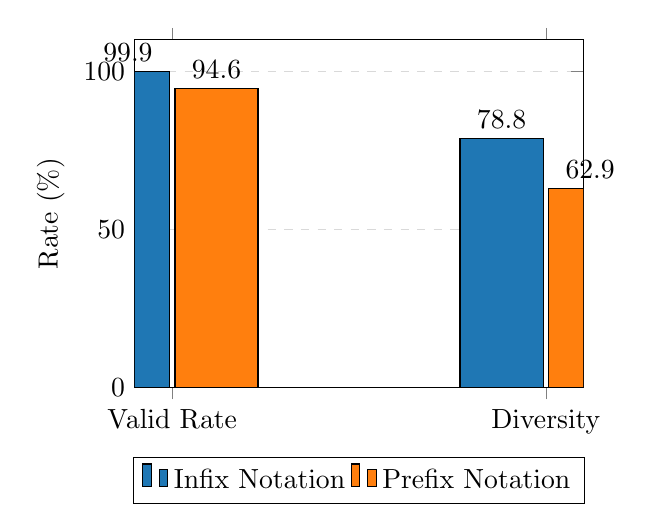
\begin{tikzpicture}
\begin{axis}[
    ybar,
    bar width=30pt,
    width=0.6\textwidth,
    height=6cm,
    ylabel={Rate (\%)},
    symbolic x coords={Valid Rate, Diversity},
    xtick=data,
    ymin=0, ymax=110,
    legend style={at={(0.5,-0.2)}, anchor=north, legend columns=2},
    nodes near coords,
    nodes near coords style={font=\normalsize, above},
    every node near coord/.append style={/pgf/number format/.cd, fixed, precision=1},
    ymajorgrids=true,
    grid style={dashed,gray!30},
]
\addplot[fill=infixcolor] coordinates {(Valid Rate, 99.9) (Diversity, 78.8)};
\addplot[fill=prefixcolor] coordinates {(Valid Rate, 94.6) (Diversity, 62.9)};
\legend{Infix Notation, Prefix Notation}
\end{axis}
\end{tikzpicture}
\caption{Notation format comparison. Infix notation achieves +5.3 pp higher valid rate and +15.9 pp higher diversity than prefix notation.}
\label{fig:notation_comparison}
\end{figure}

%==============================================================================
% FIGURE 3: Temperature Trade-off
%==============================================================================
\begin{figure}[htbp]
\centering
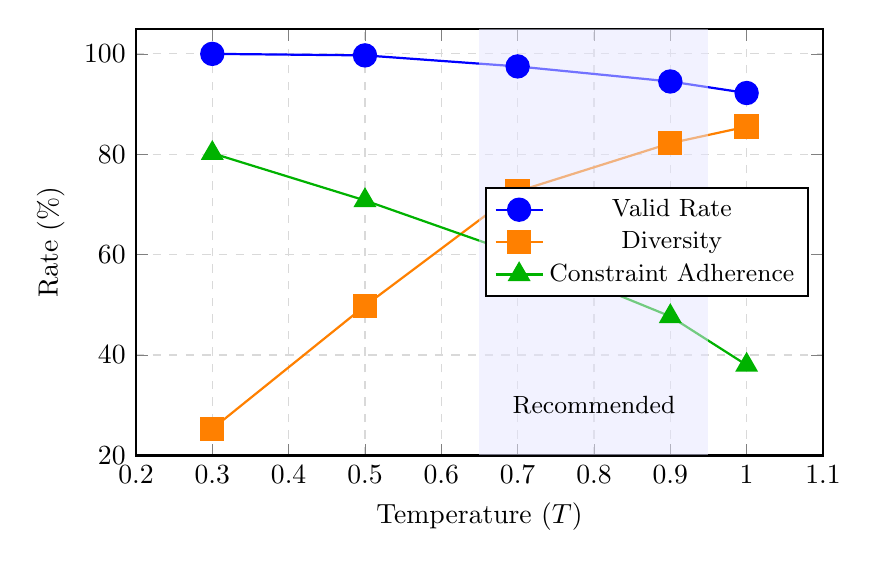
\begin{tikzpicture}
\begin{axis}[
    width=0.85\textwidth,
    height=7cm,
    xlabel={Temperature ($T$)},
    ylabel={Rate (\%)},
    xmin=0.2, xmax=1.1,
    ymin=20, ymax=105,
    legend style={at={(0.98,0.5)}, anchor=east, font=\small},
    grid=major,
    grid style={dashed,gray!30},
    mark size=4pt,
    thick,
]
\addplot[color=blue, mark=*] coordinates {
    (0.3, 100.0) (0.5, 99.7) (0.7, 97.5) (0.9, 94.5) (1.0, 92.2)
};
\addplot[color=orange, mark=square*] coordinates {
    (0.3, 25.3) (0.5, 49.8) (0.7, 72.6) (0.9, 82.2) (1.0, 85.5)
};
\addplot[color=green!70!black, mark=triangle*] coordinates {
    (0.3, 80.2) (0.5, 70.8) (0.7, 60.1) (0.9, 47.7) (1.0, 38.0)
};

% Add shaded region for recommended range
\fill[blue!10, opacity=0.5] (axis cs:0.65,20) rectangle (axis cs:0.95,105);
\node[font=\small] at (axis cs:0.8,30) {Recommended};

\legend{Valid Rate, Diversity, Constraint Adherence}
\end{axis}
\end{tikzpicture}
\caption{Temperature effect on generation quality. Shaded region ($T=0.7$--$0.9$) represents recommended operating range balancing validity and diversity.}
\label{fig:temperature_tradeoff}
\end{figure}

%==============================================================================
% FIGURE 4: Scaling Behavior
%==============================================================================
\begin{figure}[htbp]
\centering
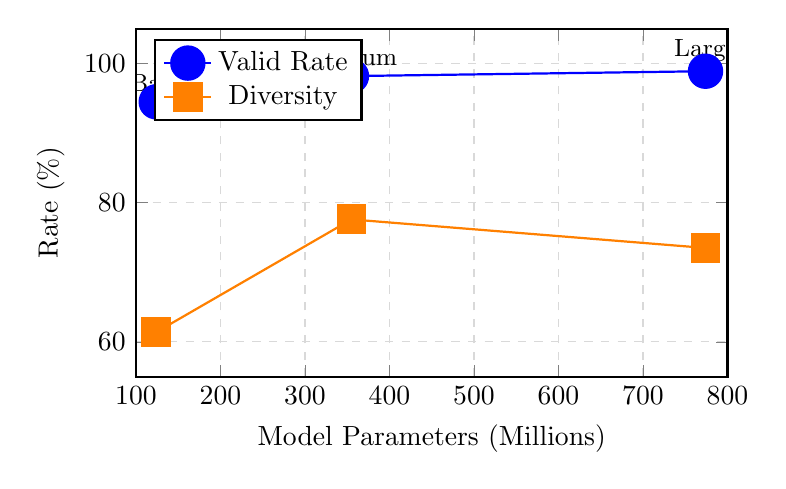
\begin{tikzpicture}
\begin{axis}[
    width=0.75\textwidth,
    height=6cm,
    xlabel={Model Parameters (Millions)},
    ylabel={Rate (\%)},
    xmin=100, xmax=800,
    ymin=55, ymax=105,
    legend style={at={(0.03,0.97)}, anchor=north west},
    grid=major,
    grid style={dashed,gray!30},
    mark size=5pt,
    thick,
]
\addplot[color=blue, mark=*, mark size=6pt] coordinates {
    (124, 94.5) (355, 98.2) (774, 98.9)
};
\addplot[color=orange, mark=square*, mark size=5pt] coordinates {
    (124, 61.4) (355, 77.6) (774, 73.5)
};
% Add labels
\node[above, font=\small] at (axis cs:124,94.5) {Base};
\node[above, font=\small] at (axis cs:355,98.2) {Medium};
\node[above, font=\small] at (axis cs:774,98.9) {Large};
\legend{Valid Rate, Diversity}
\end{axis}
\end{tikzpicture}
\caption{Model scaling behavior. Valid rate increases with model size. Diversity peaks at Medium (355M parameters).}
\label{fig:scaling}
\end{figure}

%==============================================================================
% FIGURE 5: Temperature by Model (Detailed)
%==============================================================================
\begin{figure}[htbp]
\centering
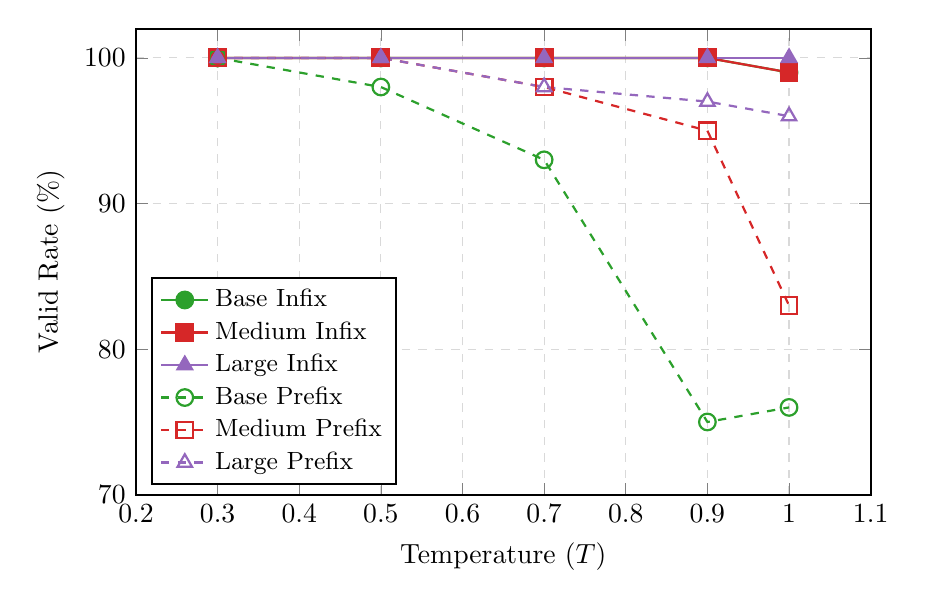
\begin{tikzpicture}
\begin{axis}[
    width=0.9\textwidth,
    height=7.5cm,
    xlabel={Temperature ($T$)},
    ylabel={Valid Rate (\%)},
    xmin=0.2, xmax=1.1,
    ymin=70, ymax=102,
    legend style={at={(0.02,0.02)}, anchor=south west, font=\small, cells={anchor=west}},
    grid=major,
    grid style={dashed,gray!30},
    mark size=3pt,
    thick,
]
% Infix models (solid lines)
\addplot[color=basecolor, mark=*] coordinates {
    (0.3, 100) (0.5, 100) (0.7, 100) (0.9, 100) (1.0, 99)
};
\addplot[color=mediumcolor, mark=square*] coordinates {
    (0.3, 100) (0.5, 100) (0.7, 100) (0.9, 100) (1.0, 99)
};
\addplot[color=largecolor, mark=triangle*] coordinates {
    (0.3, 100) (0.5, 100) (0.7, 100) (0.9, 100) (1.0, 100)
};
% Prefix models (dashed lines)
\addplot[color=basecolor, dashed, mark=o, mark options={solid}] coordinates {
    (0.3, 100) (0.5, 98) (0.7, 93) (0.9, 75) (1.0, 76)
};
\addplot[color=mediumcolor, dashed, mark=square, mark options={solid}] coordinates {
    (0.3, 100) (0.5, 100) (0.7, 98) (0.9, 95) (1.0, 83)
};
\addplot[color=largecolor, dashed, mark=triangle, mark options={solid}] coordinates {
    (0.3, 100) (0.5, 100) (0.7, 98) (0.9, 97) (1.0, 96)
};
\legend{Base Infix, Medium Infix, Large Infix, Base Prefix, Medium Prefix, Large Prefix}
\end{axis}
\end{tikzpicture}
\caption{Valid rate vs. temperature by model configuration. Solid lines represent infix models; dashed lines represent prefix models. Infix models maintain stability across temperatures.}
\label{fig:temp_by_model}
\end{figure}

%==============================================================================
% FIGURE 6: Prompt Complexity Effect
%==============================================================================
\begin{figure}[htbp]
\centering
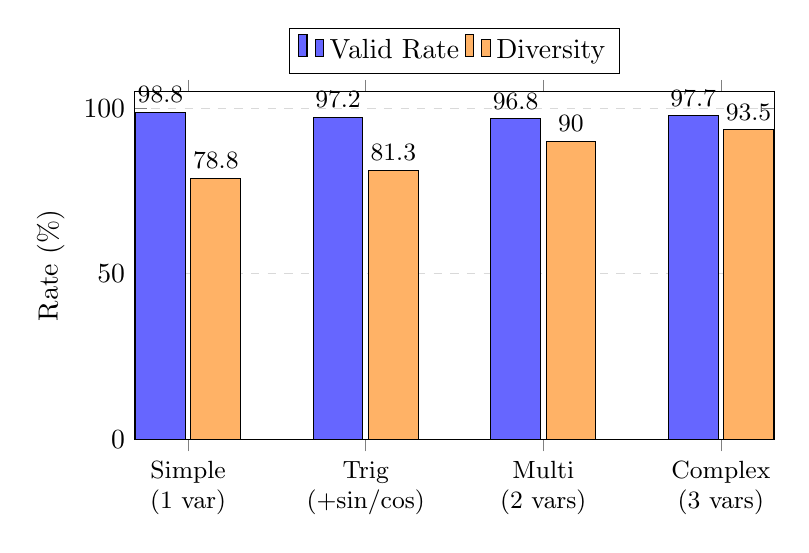
\begin{tikzpicture}
\begin{axis}[
    ybar,
    bar width=18pt,
    width=0.8\textwidth,
    height=6cm,
    ylabel={Rate (\%)},
    symbolic x coords={Simple, Trig, Multi, Complex},
    xtick=data,
    xticklabels={Simple\\(1 var), Trig\\(+sin/cos), Multi\\(2 vars), Complex\\(3 vars)},
    x tick label style={align=center, font=\small},
    ymin=0, ymax=105,
    legend style={at={(0.5,1.05)}, anchor=south, legend columns=2},
    nodes near coords,
    nodes near coords style={font=\small},
    every node near coord/.append style={/pgf/number format/.cd, fixed, precision=1},
    ymajorgrids=true,
    grid style={dashed,gray!30},
]
\addplot[fill=blue!60] coordinates {
    (Simple, 98.8) (Trig, 97.2) (Multi, 96.8) (Complex, 97.7)
};
\addplot[fill=orange!60] coordinates {
    (Simple, 78.8) (Trig, 81.3) (Multi, 90.0) (Complex, 93.5)
};
\legend{Valid Rate, Diversity}
\end{axis}
\end{tikzpicture}
\caption{Effect of prompt complexity on generation quality. More variables and operators increase expression diversity with minimal impact on validity.}
\label{fig:prompt_complexity}
\end{figure}

%==============================================================================
% FIGURE 7: Validity-Diversity Pareto Front
%==============================================================================
\begin{figure}[htbp]
\centering
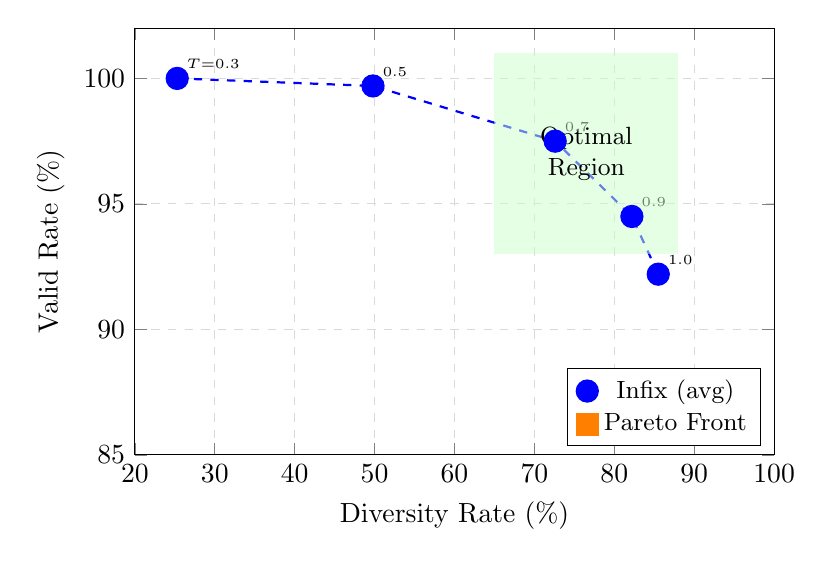
\begin{tikzpicture}
\begin{axis}[
    width=0.8\textwidth,
    height=7cm,
    xlabel={Diversity Rate (\%)},
    ylabel={Valid Rate (\%)},
    xmin=20, xmax=100,
    ymin=85, ymax=102,
    legend style={at={(0.98,0.02)}, anchor=south east, font=\small},
    grid=major,
    grid style={dashed,gray!30},
    scatter/classes={
        infix={mark=*, blue},
        prefix={mark=square*, orange}
    },
]
% Infix models at different temperatures
\addplot[scatter, only marks, scatter src=explicit symbolic, mark size=4pt]
coordinates {
    (25.3, 100.0) [infix]  % T=0.3
    (49.8, 99.7) [infix]   % T=0.5
    (72.6, 97.5) [infix]   % T=0.7
    (82.2, 94.5) [infix]   % T=0.9
    (85.5, 92.2) [infix]   % T=1.0
};
% Labels for temperatures
\node[font=\tiny, above right] at (axis cs:25.3,100) {$T$=0.3};
\node[font=\tiny, above right] at (axis cs:49.8,99.7) {0.5};
\node[font=\tiny, above right] at (axis cs:72.6,97.5) {0.7};
\node[font=\tiny, above right] at (axis cs:82.2,94.5) {0.9};
\node[font=\tiny, above right] at (axis cs:85.5,92.2) {1.0};

% Draw Pareto front
\addplot[blue, thick, dashed, no markers] coordinates {
    (25.3, 100.0) (49.8, 99.7) (72.6, 97.5) (82.2, 94.5) (85.5, 92.2)
};

% Highlight optimal region
\fill[green!20, opacity=0.5] (axis cs:65,93) rectangle (axis cs:88,101);
\node[font=\small, align=center] at (axis cs:76.5,97) {Optimal\\Region};

\legend{Infix (avg), Pareto Front}
\end{axis}
\end{tikzpicture}
\caption{Validity-diversity trade-off across temperature settings. The Pareto front shows the optimal trade-off achievable. Green region indicates recommended operating range.}
\label{fig:pareto}
\end{figure}

%==============================================================================
% FIGURE 8: Heatmap - Valid Rate by Model and Temperature
%==============================================================================
\begin{figure}[htbp]
\centering
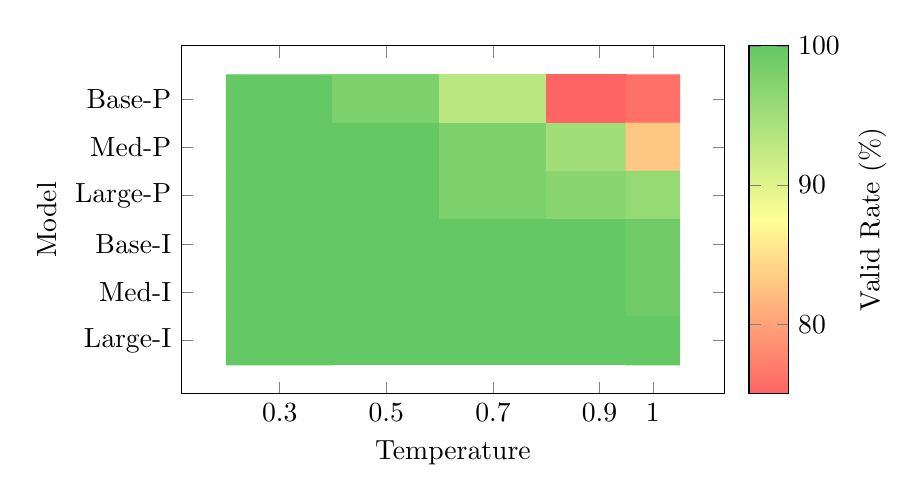
\begin{tikzpicture}
\begin{axis}[
    view={0}{90},
    colormap={validmap}{
        rgb255(0cm)=(255,100,100);
        rgb255(0.5cm)=(255,255,150);
        rgb255(1cm)=(100,200,100)
    },
    colorbar,
    colorbar style={
        ylabel={Valid Rate (\%)},
    },
    point meta min=75,
    point meta max=100,
    xlabel={Temperature},
    ylabel={Model},
    xtick={0.3, 0.5, 0.7, 0.9, 1.0},
    ytick={1,2,3,4,5,6},
    yticklabels={Base-P, Med-P, Large-P, Base-I, Med-I, Large-I},
    width=0.7\textwidth,
    height=6cm,
]
\addplot[
    matrix plot,
    mesh/cols=5,
    point meta=explicit,
] table[meta=C] {
x       y   C
0.3     1   100
0.5     1   98
0.7     1   93
0.9     1   75
1.0     1   76
0.3     2   100
0.5     2   100
0.7     2   98
0.9     2   95
1.0     2   83
0.3     3   100
0.5     3   100
0.7     3   98
0.9     3   97
1.0     3   96
0.3     4   100
0.5     4   100
0.7     4   100
0.9     4   100
1.0     4   99
0.3     5   100
0.5     5   100
0.7     5   100
0.9     5   100
1.0     5   99
0.3     6   100
0.5     6   100
0.7     6   100
0.9     6   100
1.0     6   100
};
\end{axis}
\end{tikzpicture}
\caption{Heatmap of valid rate by model and temperature. Green indicates high validity ($\geq$97\%), yellow moderate (90--97\%), red lower ($<$90\%). Infix models (top 3 rows) maintain stability.}
\label{fig:heatmap}
\end{figure}


% Color definitions (include if not already defined)
\ifx\infixcolor\undefined
\definecolor{infixcolor}{RGB}{31, 119, 180}
\definecolor{prefixcolor}{RGB}{255, 127, 14}
\definecolor{basecolor}{RGB}{44, 160, 44}
\definecolor{mediumcolor}{RGB}{214, 39, 40}
\definecolor{largecolor}{RGB}{148, 103, 189}
\fi

%==============================================================================
% FIGURE 1: Model Comparison Bar Chart
%==============================================================================
\begin{figure}[htbp]
\centering
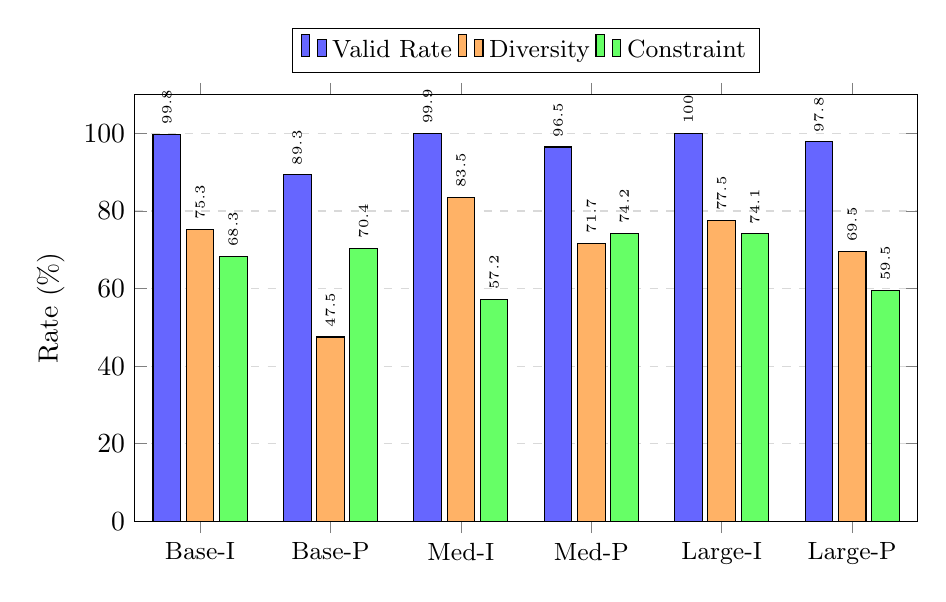
\begin{tikzpicture}
\begin{axis}[
    ybar,
    bar width=10pt,
    width=0.95\textwidth,
    height=7cm,
    ylabel={Rate (\%)},
    symbolic x coords={Base-I, Base-P, Med-I, Med-P, Large-I, Large-P},
    xtick=data,
    x tick label style={font=\small},
    ymin=0, ymax=110,
    legend style={at={(0.5,1.05)}, anchor=south, legend columns=3, font=\small},
    nodes near coords,
    nodes near coords style={font=\tiny, rotate=90, anchor=west},
    every node near coord/.append style={/pgf/number format/.cd, fixed, precision=1},
    ymajorgrids=true,
    grid style={dashed,gray!30},
]
\addplot[fill=blue!60] coordinates {
    (Base-I, 99.8) (Base-P, 89.3)
    (Med-I, 99.9) (Med-P, 96.5)
    (Large-I, 100.0) (Large-P, 97.8)
};
\addplot[fill=orange!60] coordinates {
    (Base-I, 75.3) (Base-P, 47.5)
    (Med-I, 83.5) (Med-P, 71.7)
    (Large-I, 77.5) (Large-P, 69.5)
};
\addplot[fill=green!60] coordinates {
    (Base-I, 68.3) (Base-P, 70.4)
    (Med-I, 57.2) (Med-P, 74.2)
    (Large-I, 74.1) (Large-P, 59.5)
};
\legend{Valid Rate, Diversity, Constraint}
\end{axis}
\end{tikzpicture}
\caption{Performance metrics across all model configurations. I=Infix, P=Prefix. Infix models consistently outperform prefix models in validity and diversity.}
\label{fig:model_comparison_bar}
\end{figure}

%==============================================================================
% FIGURE 2: Infix vs Prefix Comparison
%==============================================================================
\begin{figure}[htbp]
\centering
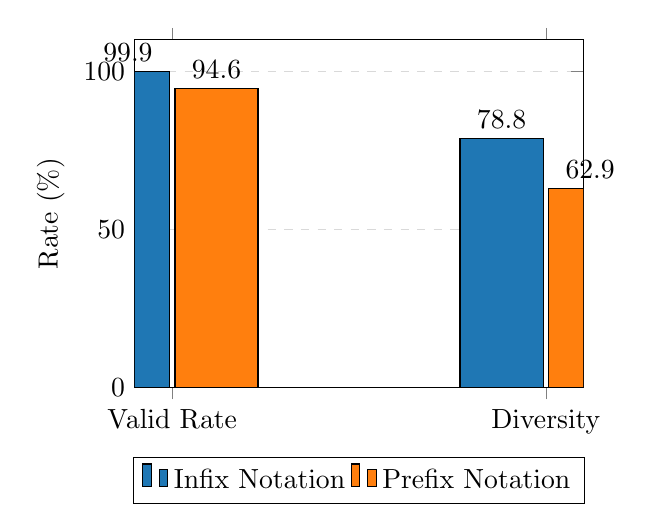
\begin{tikzpicture}
\begin{axis}[
    ybar,
    bar width=30pt,
    width=0.6\textwidth,
    height=6cm,
    ylabel={Rate (\%)},
    symbolic x coords={Valid Rate, Diversity},
    xtick=data,
    ymin=0, ymax=110,
    legend style={at={(0.5,-0.2)}, anchor=north, legend columns=2},
    nodes near coords,
    nodes near coords style={font=\normalsize, above},
    every node near coord/.append style={/pgf/number format/.cd, fixed, precision=1},
    ymajorgrids=true,
    grid style={dashed,gray!30},
]
\addplot[fill=infixcolor] coordinates {(Valid Rate, 99.9) (Diversity, 78.8)};
\addplot[fill=prefixcolor] coordinates {(Valid Rate, 94.6) (Diversity, 62.9)};
\legend{Infix Notation, Prefix Notation}
\end{axis}
\end{tikzpicture}
\caption{Notation format comparison. Infix notation achieves +5.3 pp higher valid rate and +15.9 pp higher diversity than prefix notation.}
\label{fig:notation_comparison}
\end{figure}

%==============================================================================
% FIGURE 3: Temperature Trade-off
%==============================================================================
\begin{figure}[htbp]
\centering
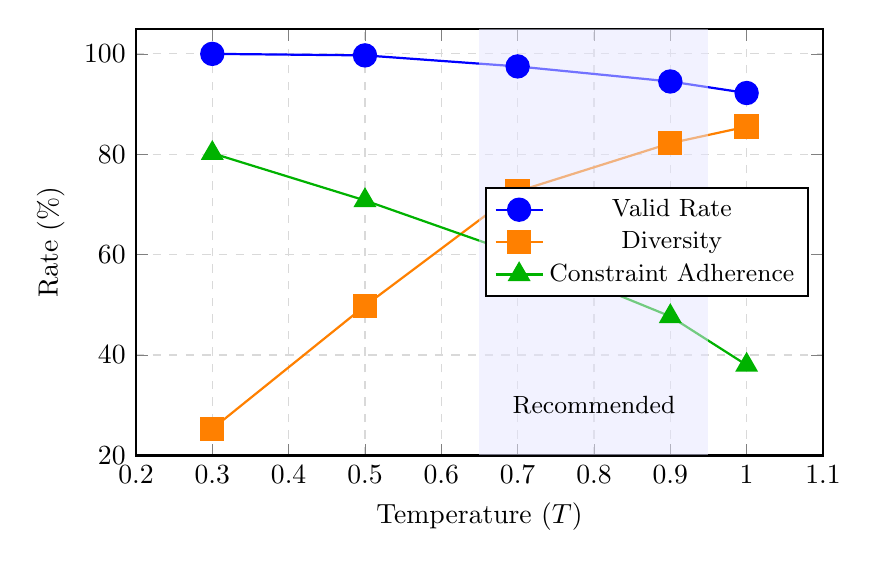
\begin{tikzpicture}
\begin{axis}[
    width=0.85\textwidth,
    height=7cm,
    xlabel={Temperature ($T$)},
    ylabel={Rate (\%)},
    xmin=0.2, xmax=1.1,
    ymin=20, ymax=105,
    legend style={at={(0.98,0.5)}, anchor=east, font=\small},
    grid=major,
    grid style={dashed,gray!30},
    mark size=4pt,
    thick,
]
\addplot[color=blue, mark=*] coordinates {
    (0.3, 100.0) (0.5, 99.7) (0.7, 97.5) (0.9, 94.5) (1.0, 92.2)
};
\addplot[color=orange, mark=square*] coordinates {
    (0.3, 25.3) (0.5, 49.8) (0.7, 72.6) (0.9, 82.2) (1.0, 85.5)
};
\addplot[color=green!70!black, mark=triangle*] coordinates {
    (0.3, 80.2) (0.5, 70.8) (0.7, 60.1) (0.9, 47.7) (1.0, 38.0)
};

% Add shaded region for recommended range
\fill[blue!10, opacity=0.5] (axis cs:0.65,20) rectangle (axis cs:0.95,105);
\node[font=\small] at (axis cs:0.8,30) {Recommended};

\legend{Valid Rate, Diversity, Constraint Adherence}
\end{axis}
\end{tikzpicture}
\caption{Temperature effect on generation quality. Shaded region ($T=0.7$--$0.9$) represents recommended operating range balancing validity and diversity.}
\label{fig:temperature_tradeoff}
\end{figure}

%==============================================================================
% FIGURE 4: Scaling Behavior
%==============================================================================
\begin{figure}[htbp]
\centering
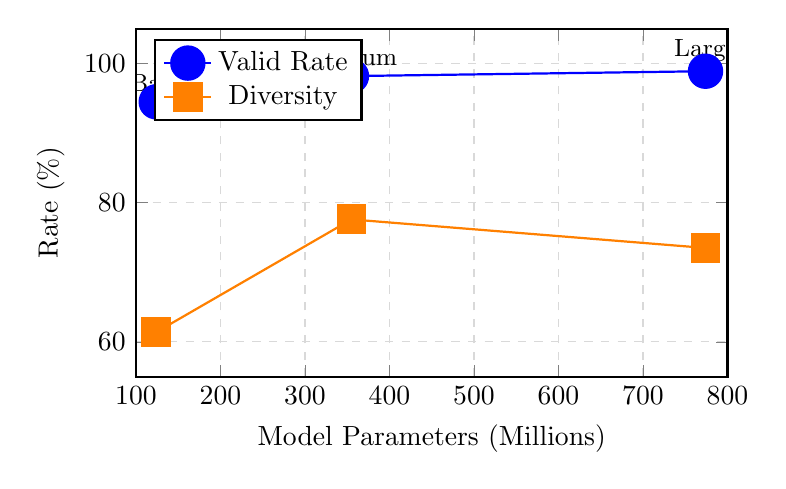
\begin{tikzpicture}
\begin{axis}[
    width=0.75\textwidth,
    height=6cm,
    xlabel={Model Parameters (Millions)},
    ylabel={Rate (\%)},
    xmin=100, xmax=800,
    ymin=55, ymax=105,
    legend style={at={(0.03,0.97)}, anchor=north west},
    grid=major,
    grid style={dashed,gray!30},
    mark size=5pt,
    thick,
]
\addplot[color=blue, mark=*, mark size=6pt] coordinates {
    (124, 94.5) (355, 98.2) (774, 98.9)
};
\addplot[color=orange, mark=square*, mark size=5pt] coordinates {
    (124, 61.4) (355, 77.6) (774, 73.5)
};
% Add labels
\node[above, font=\small] at (axis cs:124,94.5) {Base};
\node[above, font=\small] at (axis cs:355,98.2) {Medium};
\node[above, font=\small] at (axis cs:774,98.9) {Large};
\legend{Valid Rate, Diversity}
\end{axis}
\end{tikzpicture}
\caption{Model scaling behavior. Valid rate increases with model size. Diversity peaks at Medium (355M parameters).}
\label{fig:scaling}
\end{figure}

%==============================================================================
% FIGURE 5: Temperature by Model (Detailed)
%==============================================================================
\begin{figure}[htbp]
\centering
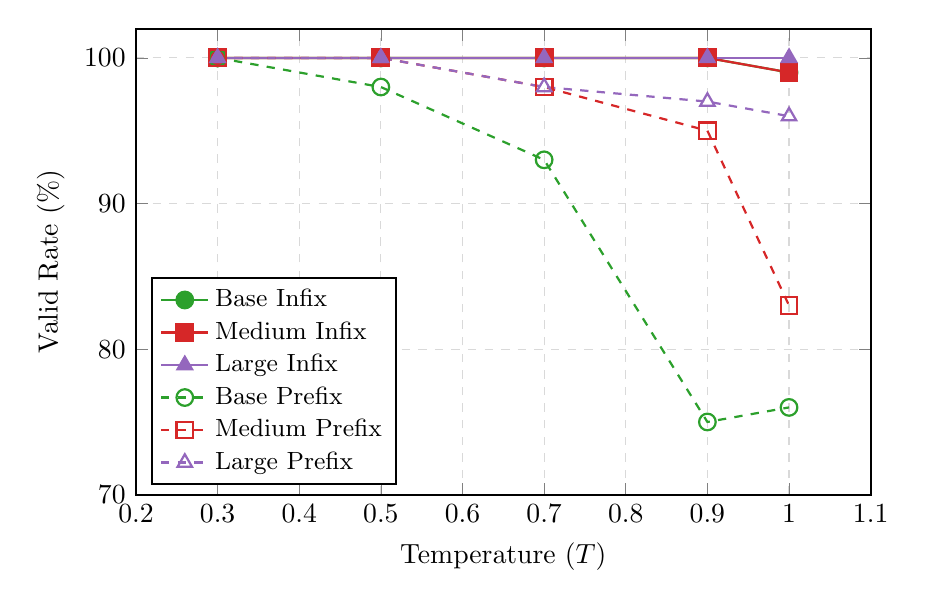
\begin{tikzpicture}
\begin{axis}[
    width=0.9\textwidth,
    height=7.5cm,
    xlabel={Temperature ($T$)},
    ylabel={Valid Rate (\%)},
    xmin=0.2, xmax=1.1,
    ymin=70, ymax=102,
    legend style={at={(0.02,0.02)}, anchor=south west, font=\small, cells={anchor=west}},
    grid=major,
    grid style={dashed,gray!30},
    mark size=3pt,
    thick,
]
% Infix models (solid lines)
\addplot[color=basecolor, mark=*] coordinates {
    (0.3, 100) (0.5, 100) (0.7, 100) (0.9, 100) (1.0, 99)
};
\addplot[color=mediumcolor, mark=square*] coordinates {
    (0.3, 100) (0.5, 100) (0.7, 100) (0.9, 100) (1.0, 99)
};
\addplot[color=largecolor, mark=triangle*] coordinates {
    (0.3, 100) (0.5, 100) (0.7, 100) (0.9, 100) (1.0, 100)
};
% Prefix models (dashed lines)
\addplot[color=basecolor, dashed, mark=o, mark options={solid}] coordinates {
    (0.3, 100) (0.5, 98) (0.7, 93) (0.9, 75) (1.0, 76)
};
\addplot[color=mediumcolor, dashed, mark=square, mark options={solid}] coordinates {
    (0.3, 100) (0.5, 100) (0.7, 98) (0.9, 95) (1.0, 83)
};
\addplot[color=largecolor, dashed, mark=triangle, mark options={solid}] coordinates {
    (0.3, 100) (0.5, 100) (0.7, 98) (0.9, 97) (1.0, 96)
};
\legend{Base Infix, Medium Infix, Large Infix, Base Prefix, Medium Prefix, Large Prefix}
\end{axis}
\end{tikzpicture}
\caption{Valid rate vs. temperature by model configuration. Solid lines represent infix models; dashed lines represent prefix models. Infix models maintain stability across temperatures.}
\label{fig:temp_by_model}
\end{figure}

%==============================================================================
% FIGURE 6: Prompt Complexity Effect
%==============================================================================
\begin{figure}[htbp]
\centering
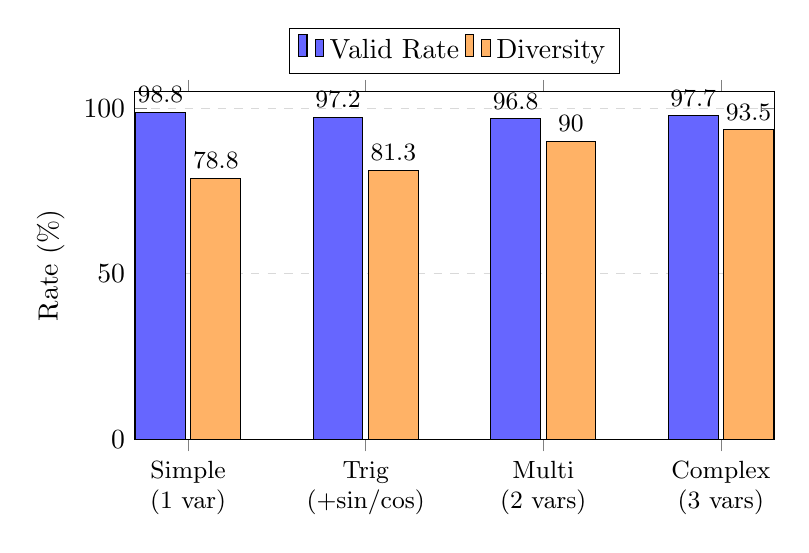
\begin{tikzpicture}
\begin{axis}[
    ybar,
    bar width=18pt,
    width=0.8\textwidth,
    height=6cm,
    ylabel={Rate (\%)},
    symbolic x coords={Simple, Trig, Multi, Complex},
    xtick=data,
    xticklabels={Simple\\(1 var), Trig\\(+sin/cos), Multi\\(2 vars), Complex\\(3 vars)},
    x tick label style={align=center, font=\small},
    ymin=0, ymax=105,
    legend style={at={(0.5,1.05)}, anchor=south, legend columns=2},
    nodes near coords,
    nodes near coords style={font=\small},
    every node near coord/.append style={/pgf/number format/.cd, fixed, precision=1},
    ymajorgrids=true,
    grid style={dashed,gray!30},
]
\addplot[fill=blue!60] coordinates {
    (Simple, 98.8) (Trig, 97.2) (Multi, 96.8) (Complex, 97.7)
};
\addplot[fill=orange!60] coordinates {
    (Simple, 78.8) (Trig, 81.3) (Multi, 90.0) (Complex, 93.5)
};
\legend{Valid Rate, Diversity}
\end{axis}
\end{tikzpicture}
\caption{Effect of prompt complexity on generation quality. More variables and operators increase expression diversity with minimal impact on validity.}
\label{fig:prompt_complexity}
\end{figure}

%==============================================================================
% FIGURE 7: Validity-Diversity Pareto Front
%==============================================================================
\begin{figure}[htbp]
\centering
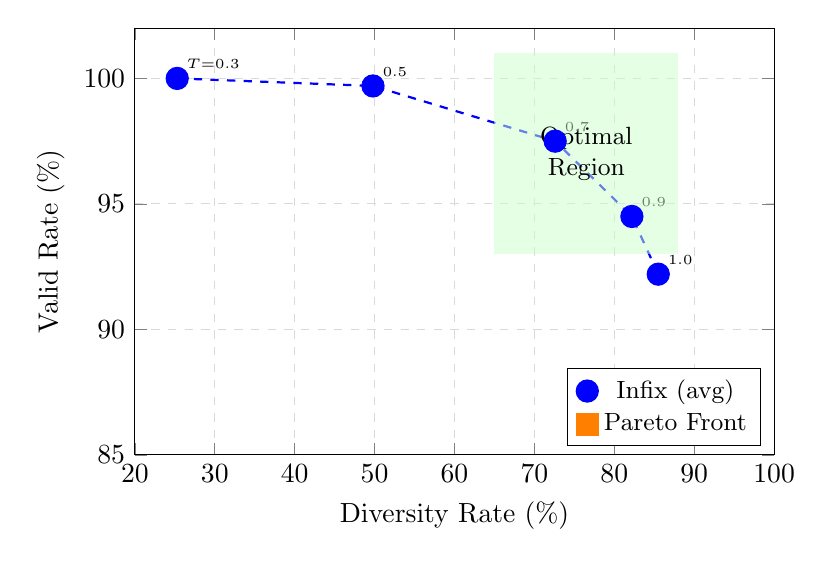
\begin{tikzpicture}
\begin{axis}[
    width=0.8\textwidth,
    height=7cm,
    xlabel={Diversity Rate (\%)},
    ylabel={Valid Rate (\%)},
    xmin=20, xmax=100,
    ymin=85, ymax=102,
    legend style={at={(0.98,0.02)}, anchor=south east, font=\small},
    grid=major,
    grid style={dashed,gray!30},
    scatter/classes={
        infix={mark=*, blue},
        prefix={mark=square*, orange}
    },
]
% Infix models at different temperatures
\addplot[scatter, only marks, scatter src=explicit symbolic, mark size=4pt]
coordinates {
    (25.3, 100.0) [infix]  % T=0.3
    (49.8, 99.7) [infix]   % T=0.5
    (72.6, 97.5) [infix]   % T=0.7
    (82.2, 94.5) [infix]   % T=0.9
    (85.5, 92.2) [infix]   % T=1.0
};
% Labels for temperatures
\node[font=\tiny, above right] at (axis cs:25.3,100) {$T$=0.3};
\node[font=\tiny, above right] at (axis cs:49.8,99.7) {0.5};
\node[font=\tiny, above right] at (axis cs:72.6,97.5) {0.7};
\node[font=\tiny, above right] at (axis cs:82.2,94.5) {0.9};
\node[font=\tiny, above right] at (axis cs:85.5,92.2) {1.0};

% Draw Pareto front
\addplot[blue, thick, dashed, no markers] coordinates {
    (25.3, 100.0) (49.8, 99.7) (72.6, 97.5) (82.2, 94.5) (85.5, 92.2)
};

% Highlight optimal region
\fill[green!20, opacity=0.5] (axis cs:65,93) rectangle (axis cs:88,101);
\node[font=\small, align=center] at (axis cs:76.5,97) {Optimal\\Region};

\legend{Infix (avg), Pareto Front}
\end{axis}
\end{tikzpicture}
\caption{Validity-diversity trade-off across temperature settings. The Pareto front shows the optimal trade-off achievable. Green region indicates recommended operating range.}
\label{fig:pareto}
\end{figure}

%==============================================================================
% FIGURE 8: Heatmap - Valid Rate by Model and Temperature
%==============================================================================
\begin{figure}[htbp]
\centering
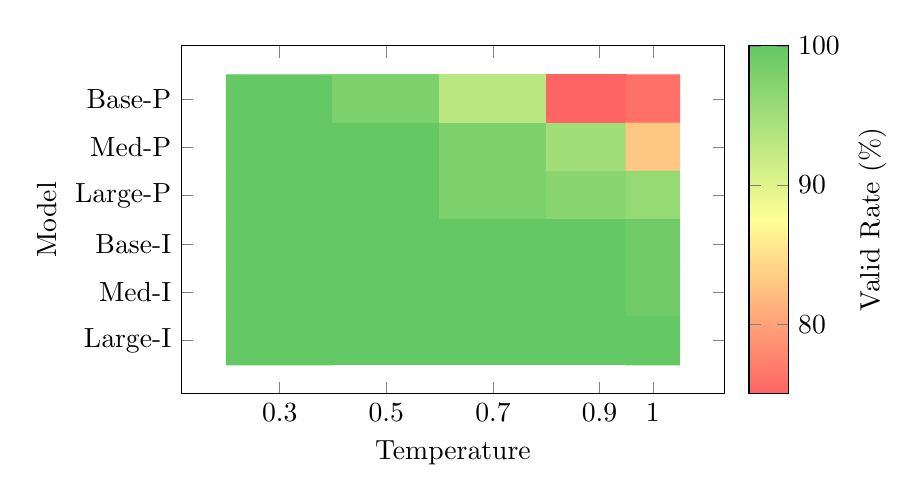
\begin{tikzpicture}
\begin{axis}[
    view={0}{90},
    colormap={validmap}{
        rgb255(0cm)=(255,100,100);
        rgb255(0.5cm)=(255,255,150);
        rgb255(1cm)=(100,200,100)
    },
    colorbar,
    colorbar style={
        ylabel={Valid Rate (\%)},
    },
    point meta min=75,
    point meta max=100,
    xlabel={Temperature},
    ylabel={Model},
    xtick={0.3, 0.5, 0.7, 0.9, 1.0},
    ytick={1,2,3,4,5,6},
    yticklabels={Base-P, Med-P, Large-P, Base-I, Med-I, Large-I},
    width=0.7\textwidth,
    height=6cm,
]
\addplot[
    matrix plot,
    mesh/cols=5,
    point meta=explicit,
] table[meta=C] {
x       y   C
0.3     1   100
0.5     1   98
0.7     1   93
0.9     1   75
1.0     1   76
0.3     2   100
0.5     2   100
0.7     2   98
0.9     2   95
1.0     2   83
0.3     3   100
0.5     3   100
0.7     3   98
0.9     3   97
1.0     3   96
0.3     4   100
0.5     4   100
0.7     4   100
0.9     4   100
1.0     4   99
0.3     5   100
0.5     5   100
0.7     5   100
0.9     5   100
1.0     5   99
0.3     6   100
0.5     6   100
0.7     6   100
0.9     6   100
1.0     6   100
};
\end{axis}
\end{tikzpicture}
\caption{Heatmap of valid rate by model and temperature. Green indicates high validity ($\geq$97\%), yellow moderate (90--97\%), red lower ($<$90\%). Infix models (top 3 rows) maintain stability.}
\label{fig:heatmap}
\end{figure}
